\documentclass[12pt]{article}

\usepackage{amssymb}
\usepackage{booktabs}
\usepackage{floatrow}
\usepackage{graphicx}
\usepackage{listings}
\usepackage{url}

\title{Anti-plagiarism Project}
\date{2015-10-21}
\author{Eric Scott Freeman}

\begin{document}
	\pagenumbering{gobble}
	\maketitle
	\newpage
	\tableofcontents
	\newpage
	\pagenumbering{arabic}
	\section{Introduction}
		The University of Stavanger uses an application called Autograder, written by Heine Furubotten, to automatically grade students' programming assignments. Autograder works with Github. Whenever a student pushes their code to Github, Autograder will pull a copy of the code and run a series of tests on it. Autograder does not currently have support for plagiarism detection. The goal of this project is to integrate a few anti-plagiarism tools into Autograder, thereby helping the professors save time.
		
	\section{Related Work}
		Unfortunately software plagiarism is a problem both in the classroom and in the workplace. A number of applications have been created to help detect this problem. While these tools can detect similarities in programs, the flagged files must still be manually examined to determine whether or not code was plagiarized.
		
		There are several different general techniques that are used to look for plagiarism. The tools analyzed in this project used either fingerprinting or stylometry.
	
		\subsection{Fingerprinting}
			Several tools use a technique called fingerprinting to detect plagiarism. In fingerprinting algorithms, hashes of $n$-grams, substrings that are $n$ characters, are saved and compared to help find plagiarism. Not all hashes are stored due to the large number that would be produced. 
		
			\subsubsection{Winnowing}
				Moss uses a technique called winnowing to select which hashes to save \cite{schleimer+wilkerson+aiken}. In the winnowing algorithm, a window, selection of contiguous hashes, is used to help select which hashes to save. The smallest hash from a window is saved, and then the window moves one hash over. The smallest hash from the next window is often the smallest hash from the previous window. If so it is not saved again. Figure \ref{fig:winnowing1} shows an example of how winnowing works. The orange box represents the shifting window. The green box shows whenever a new hash is saved.
				
				\begin{figure}[h!]
					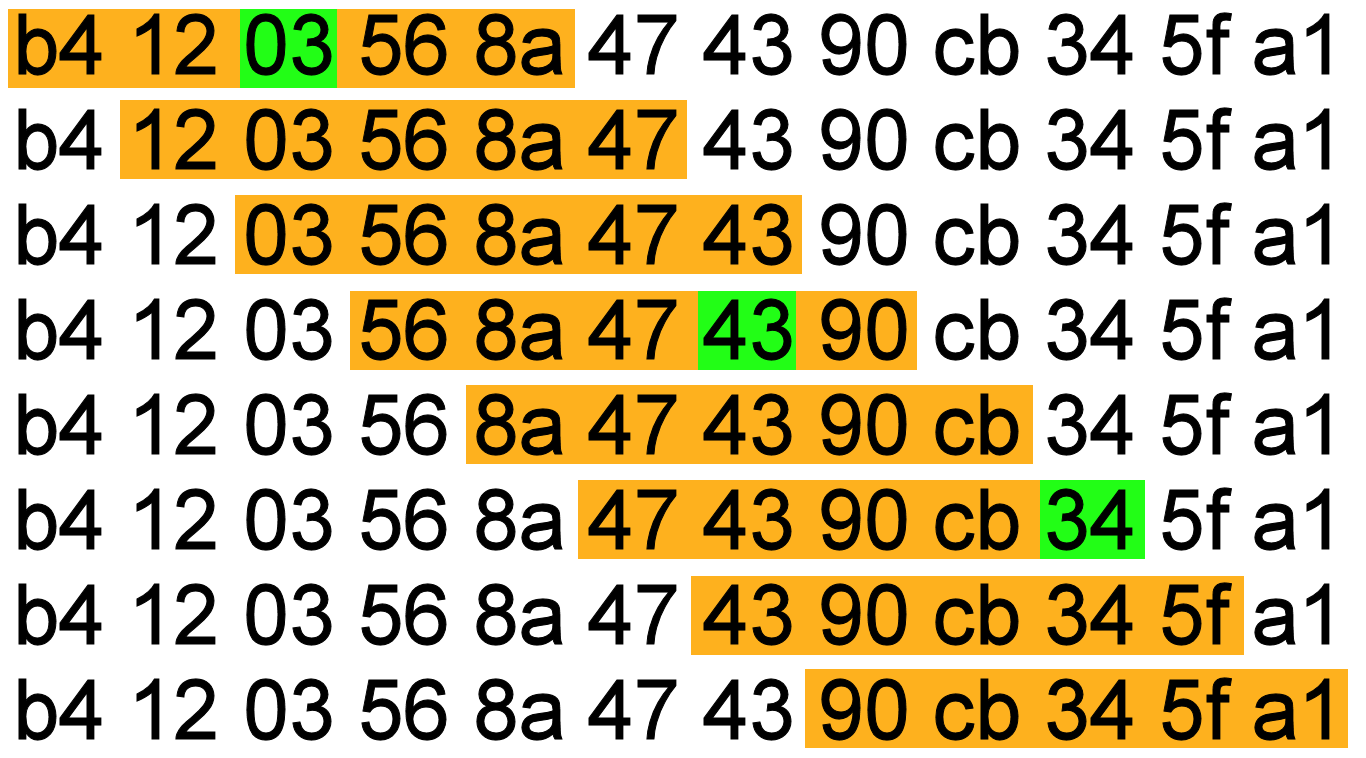
\includegraphics[width=0.6\textwidth]{Winnowing.png}
					\caption{Winnowing.}
					\label{fig:winnowing1}
				\end{figure}
			
			\subsubsection{Running-Karp-Rabin Greedy-String-Tiling}
				JPlag uses Running-Karp-Rabin Greedy-String-Tiling (RKS-GST) to compare hashes of code in plagiarism detection \cite{prechelt+malpohl+philippsen}. RKS-GST was originally used in YAP3, another plagiarism detection tool. In RKS-GST, the Greedy String half of the algorithm forms pairs of substrings, each from a different string. Then the Karp-Rabin half of the algorithm hashes each substring in the pair \cite{wise}. This is done to help detect code reordering.
		
		\subsection{Stylometry}
			Another approach is to use code stylometry, which analyzes the style of writing or coding.
			
			\subsubsection{Abstract Syntax Trees}
				Caliskan-Islam, et al. use abstract syntax trees (ASTs) to compare the styles of authors \cite{caliskan-islam+harang+liu}. Things that are easily changed in code, such as variable names, become leaves in the AST, while the structure of the tree is harder to change \cite{caliskan-islam+harang+liu}. Figure \ref{fig:ast} shows an abstract syntax tree of the code in Figure \ref{fig:astcode}. Note how the leaves, or circular nodes, in Figure \ref{fig:ast} are variable names, constants, and a function name.
				
				Michal Bohuslávek's dupl application uses ASTs to find similarities in code \cite{bohuslave}. It looks for any copies of code, not just plagiarism. So if a piece of code is duplicated even in the same file, it will test positive.
			
				\begin{figure}
					\begin{floatrow}
						\ffigbox{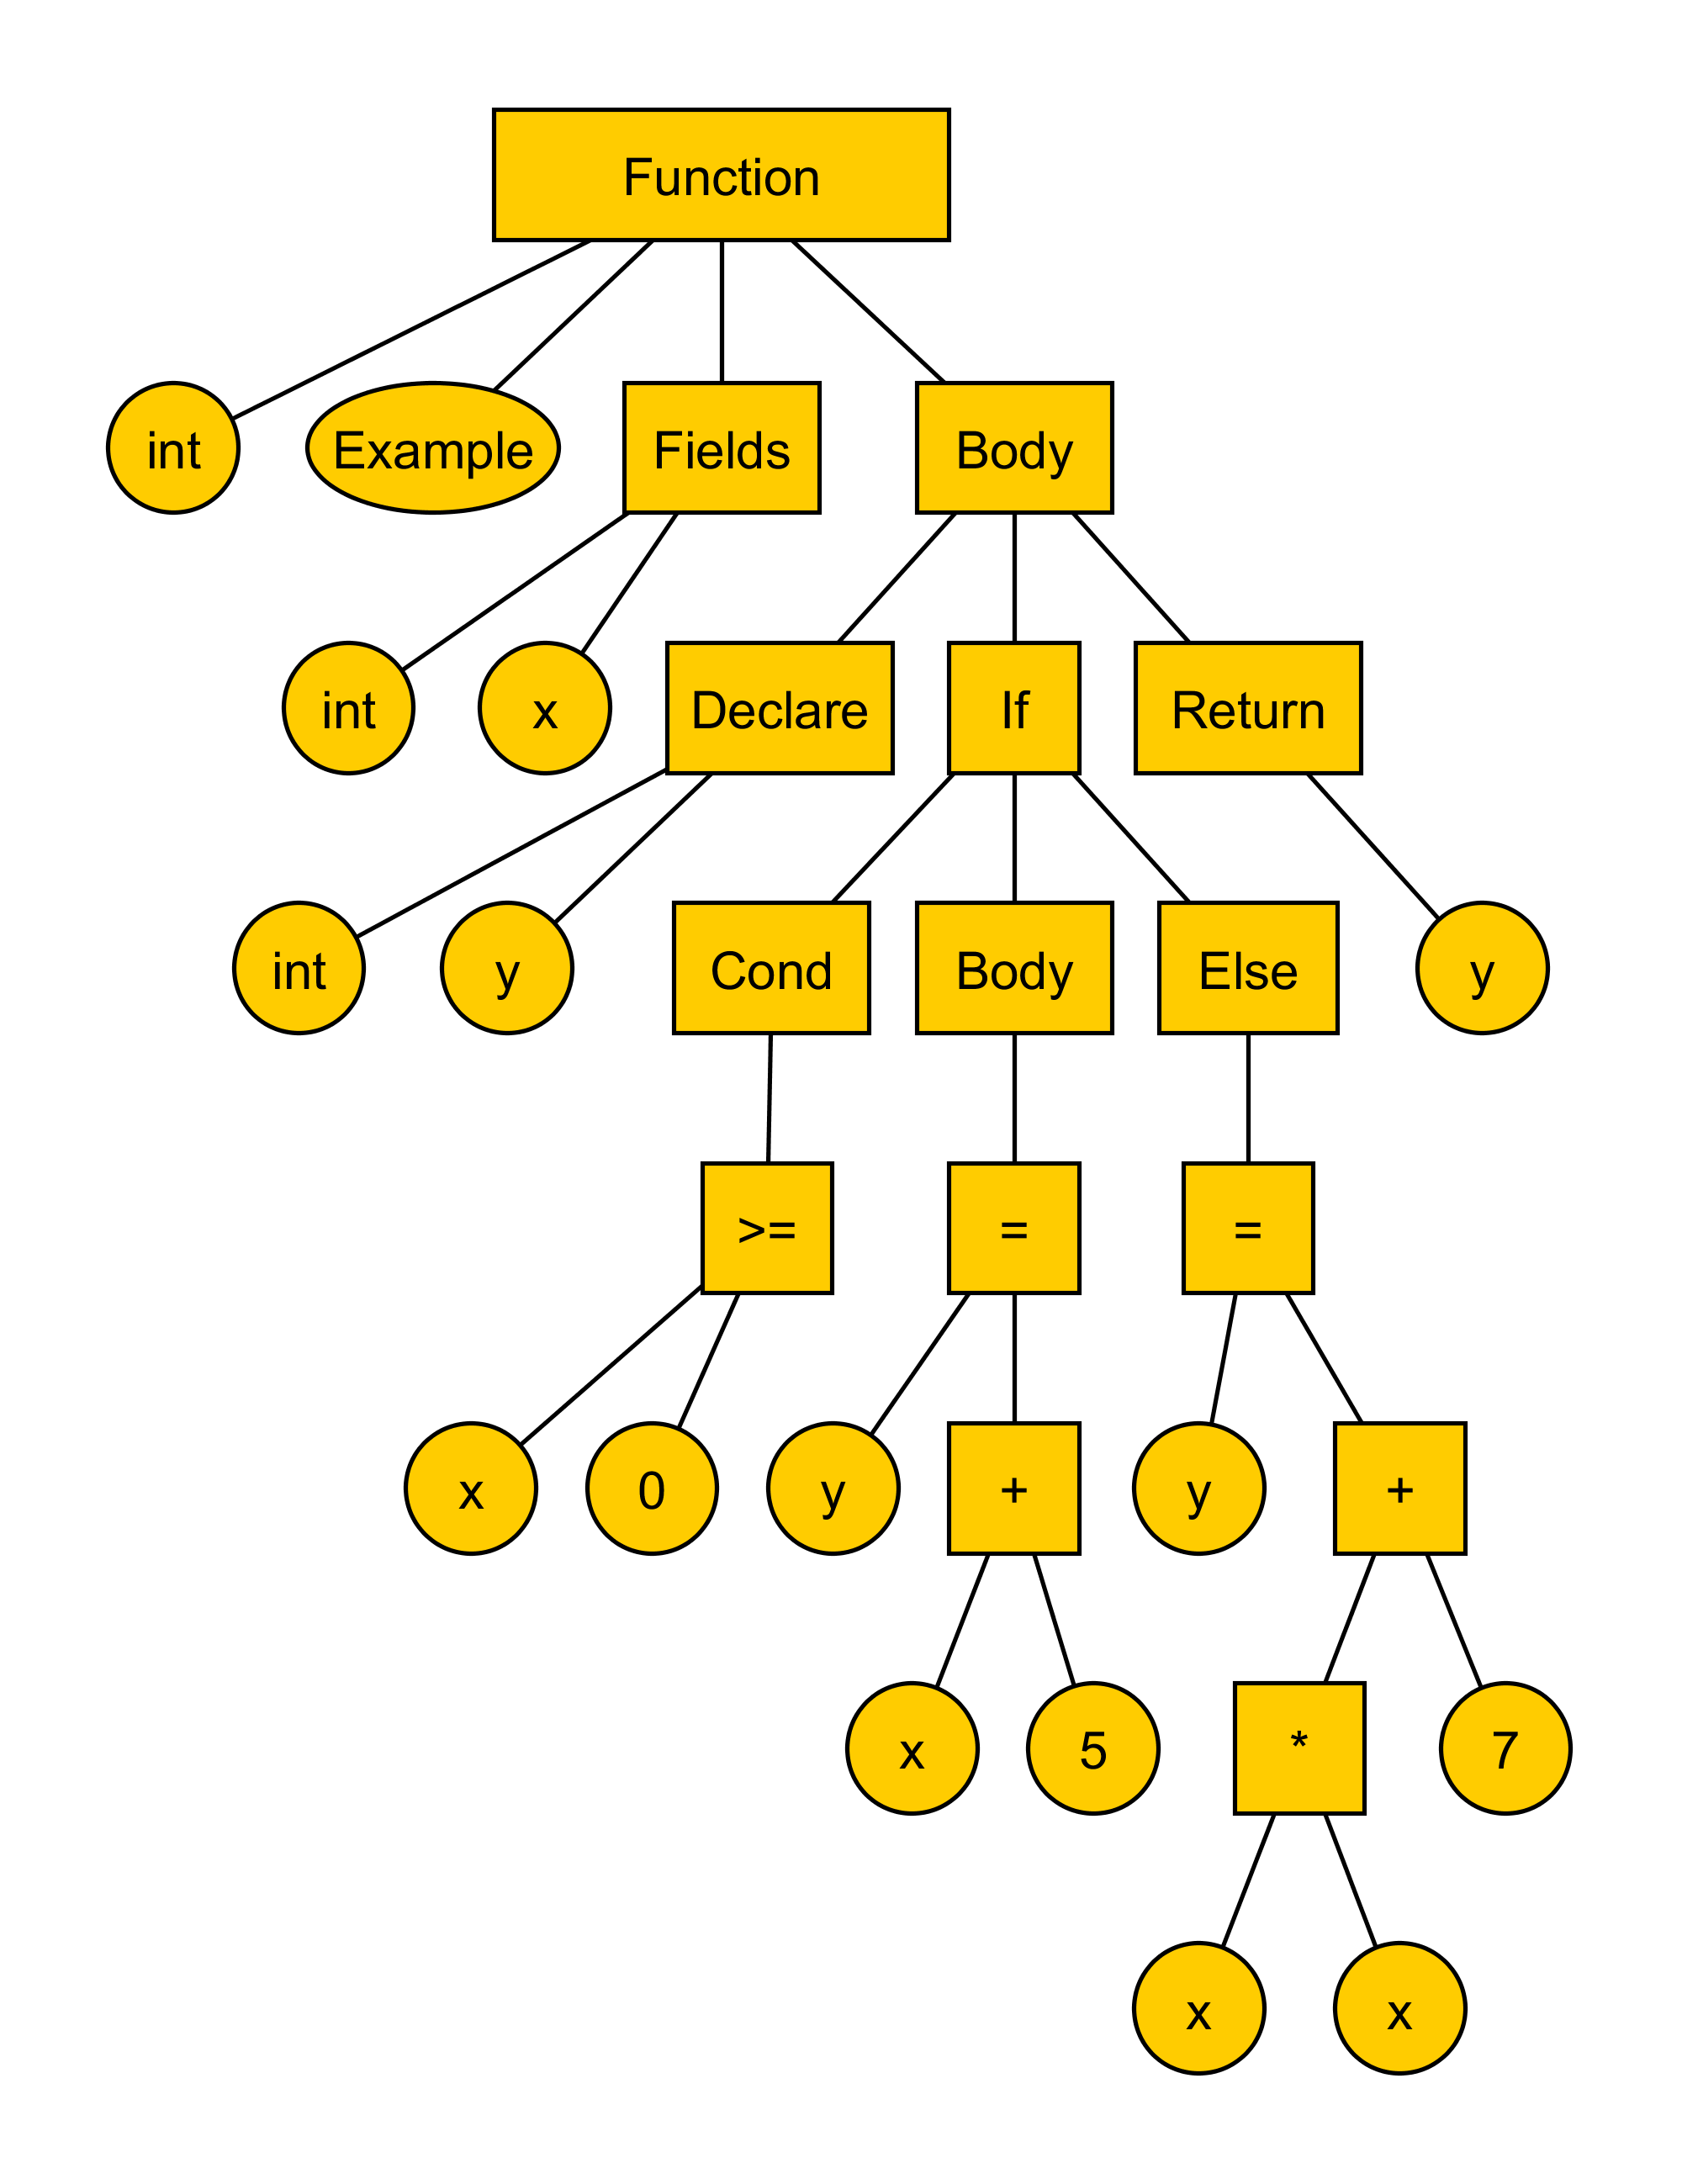
\includegraphics[width=0.5\textwidth]{AST.png}}{\caption{Abstract syntax tree.}\label{fig:ast}}	\ffigbox{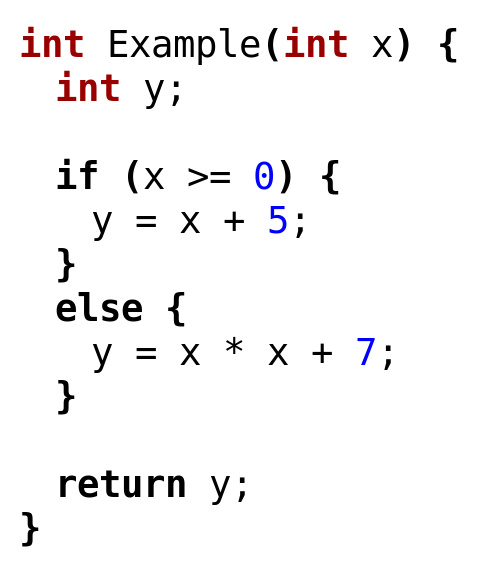
\includegraphics[width=0.3\textwidth]{ASTcode.png}}{\caption{Example code.}\label{fig:astcode}}
					\end{floatrow}
				\end{figure}
		
		\subsection{Supported Languages}
			Fingerprinting and string comparison techniques can be used to analyze source code written in languages other than their officially supported languages. Moss can analyze Go code, even though it is not technically supported. Since ASTs need to parse the code, applications which use them are stricter on which languages they can analyze. For example dupl only supports code written in Go. Table \ref{tab:languageSupport} shows the languages officially supported by several anti-plagiarism tools.
		
			\begin{table}[h!]
				\begin{center}
					\caption{Officially supported languages by various tools}
					\label{tab:languageSupport}
					\begin{tabular}{ccccccccccccccc}
						\toprule
						Tool & Java & Go & C & C\verb!++! & C\verb!#! & Python & Perl & others\\
						\midrule
						Moss & \checkmark & & \checkmark & \checkmark & \checkmark & \checkmark & \checkmark & \checkmark \\
						JPlag & \checkmark & & \checkmark & \checkmark & \checkmark & & & \checkmark\\
						Plaggie & \checkmark & & & & & & & \\
						SIM & \checkmark & & \checkmark & & & & & \checkmark\\
						dupl & & \checkmark & & & & & & \\
						\bottomrule
					\end{tabular}
				\end{center}
			\end{table}
		
	\section{Design}
		\subsection{Understanding Autograder}
			To be able to add functionality to Autograder, it was necessary to understand how it works. This meant looking through the code to see what happens when certain events occurred. For example, when the Rebuild button on the teacherresultpage.html is pressed, this calls the \verb|$("#rebuild").click()| function in the teacher.result.page.js file. The click function then posts to the /event/manualbuild URL. webserver.go handles the post by calling ManualCITriggerHandler() function in ci.go. ManualCITriggerHandler() then starts the daemon, which creates a Docker container and a set of commands to run on the docker container. The docker container pulls the students code and the test code from GitHub and proceeds to run the tests on it.	
			
		\subsection{Process}
			Since Autograder was written in Go, this project is also written in Go. Later it was decided to make this project a standalone application that Autograder will call, since another university has expressed interest in using it. The program will call each of the anti-plagiarism tools and store the results. The \verb|golint| application was run against the code for suggestions on making the code follow Go coding conventions. The \verb|go fmt| command was run to clean up the whitespace in the code. A separate Go package will be written for each anti-plagiarism tool. The packages will implement a common interface which will create the commands to send to the tools and will format the results.
			
			The anti-plagiarism application will have two main functions. The first is to call the various anti-plagiarism detection tools, and the second is to check and store the results. It can take an indefinite amount of time for the tools to complete their analysis of the students' code, so it is best for the application to run the commands for the tools as a background process by using the $\&$ symbol at the end of each command.
			
			\subsubsection{Calling the anti-plagiarism tools}
			Before calling the anti-plagiarism tools, first the students' code will be pulled from Github to the Autograder server. The directory structure will consist of a base directory containing subdirectories for each class. Inside each class, there will be directories for each student, which will have directories for each assignment. See figure \ref{fig:directories}. This is similar to how Autograder stores the files in Github, so pulling the code for the anti-plagiarism project will be simplified. Each student's work for an assignment to be compared against the other students' work for that assignment in that class. This will keep the number of files being compared from growing too large. 
			
			\begin{figure}[h!]
				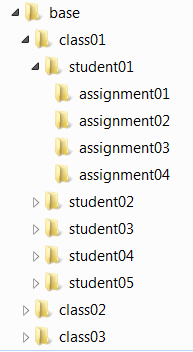
\includegraphics[width=0.2\textwidth]{Directories.png}
				\caption{Directory structure.}
				\label{fig:directories}
			\end{figure}
			
			\begin{figure}[h!]
				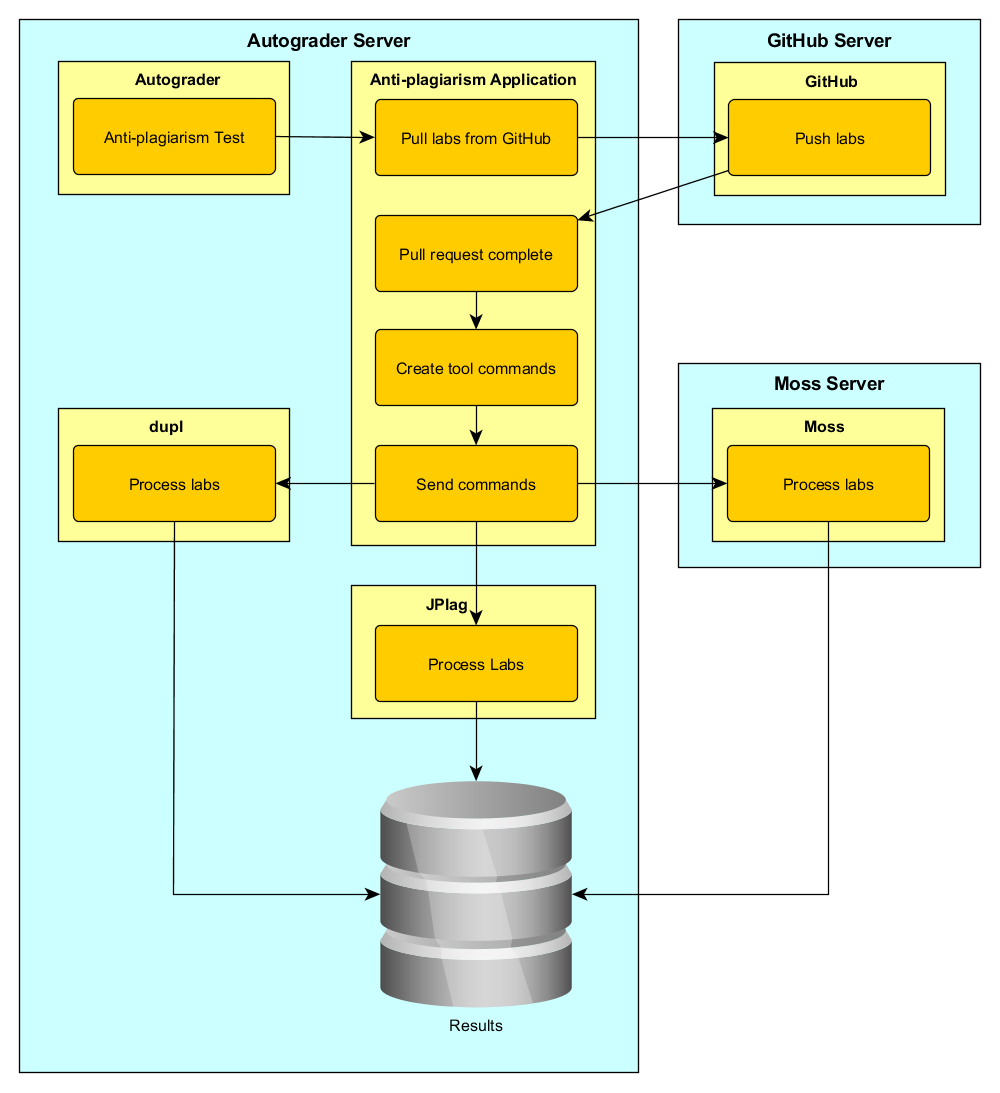
\includegraphics[width=0.7\textwidth]{step1.png}
				\caption{Step 1}
				\label{fig:step1}
			\end{figure}
			
			Next the commands are created for each anti-plagiarism tools based on the location of the code, the language in which the code was written, the threshold of the tool, and various other parameters.
			
			\subsubsection{Checking for and storing the results}
			
			\begin{figure}[h!]
				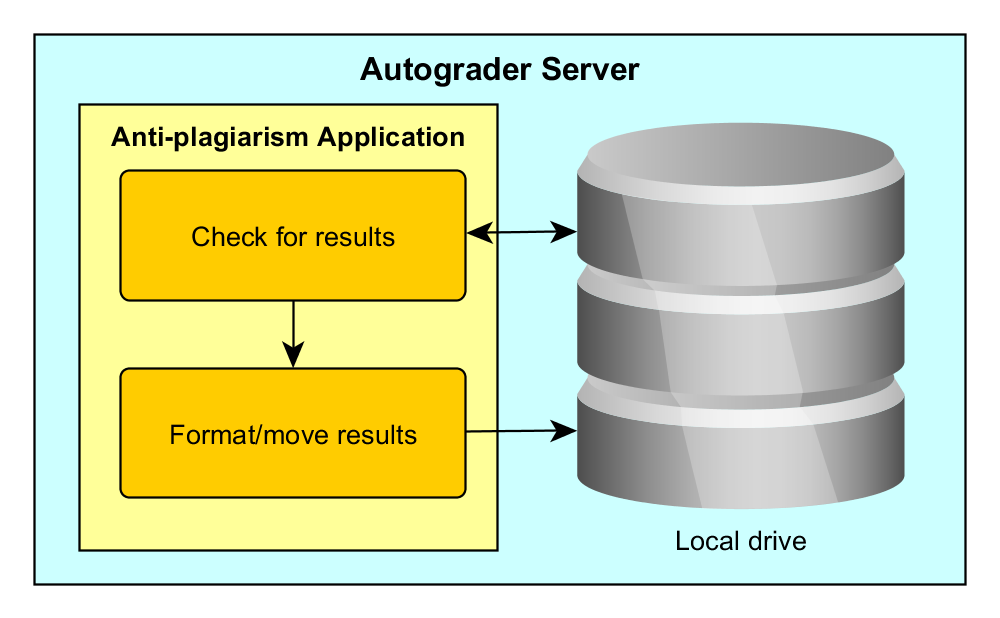
\includegraphics[width=0.7\textwidth]{step2.png}
				\caption{Step 2}
				\label{fig:step2}
			\end{figure}
			
	\section{Results}
	\section{Issues}
		A few issues were encountered during the project.
		\begin{itemize}
			\item JPlag will only work with the languages it supports. Therefore JPlag will not accept Go files. 
			\item dupl will not compare files it cannot parse. So files that are submitted with syntax errors could have plagiarized code, but they will remain unnoticed.
		\end{itemize}
	\section{Analysis}
	\section{Conclusion}
	\bibliography{sources}
	\bibliographystyle{ieeetr}
\end{document}